\documentclass[tikz,border=10pt]{standalone}
% Only TikZ is used; math mode works without extra packages.
\begin{document}
% Coordinates: origin at O (px 303.6, 264.2), scale 0.015 units/px, y flipped.
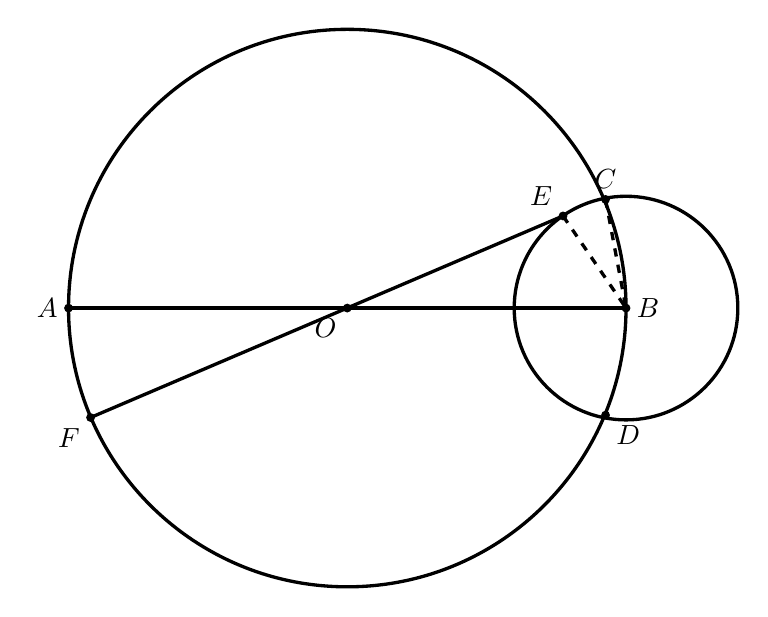
\begin{tikzpicture}[line width=1.2pt, line join=round]

% Named points
\coordinate (O) at (0,0);
\coordinate (A) at (-3.54,0);
\coordinate (B) at (3.54,0);
\coordinate (F) at (-3.26,-1.39);
\coordinate (E) at (2.74,1.17);
\coordinate (C) at (3.28,1.38);
\coordinate (D) at (3.28,-1.36);

% Big circle (center O, radius 236 px)
\draw (O) circle (3.54);

% Small circle (center B, radius 94.5 px)
\draw (B) circle (1.42);

% Solid diameter A-O-B
\draw (A) -- (B);

% Solid line F-O-E
\draw (F) -- (E);

% Dashed segments E-B and C-B
\draw[dashed] (E) -- (B);
\draw[dashed] (C) -- (B);

% Point markers
\foreach \p in {O,A,B,F,E,C,D}
  \fill (\p) circle (1.6pt);

% Labels
\node[above] at (C) {$C$};
\node[below right] at (D) {$D$};
\node[above left] at (E) {$E$};
\node[right] at (B) {$B$};
\node[left] at (A) {$A$};
\node[below left] at (O) {$O$};
\node[below left] at (F) {$F$};

\end{tikzpicture}
\end{document}